\section{Example Appendix} \label{appendix:a}
\subsection{Codes}
\subsection{Figures}
\begin{figure}[h]
    \centering
    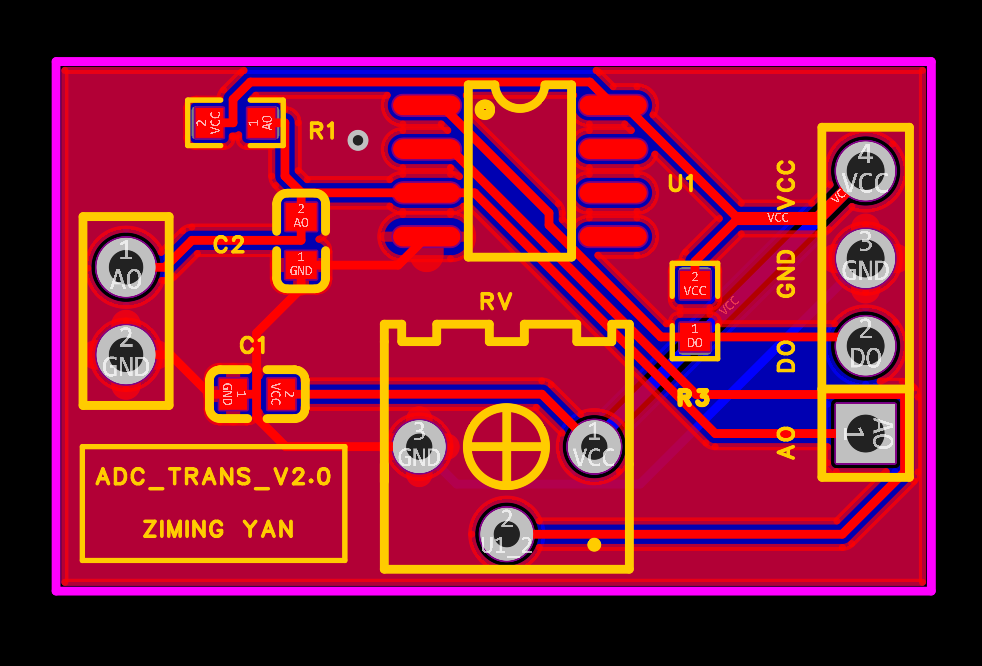
\includegraphics[width=0.8\textwidth]{Figures/FSR402_PCB.png}
    \caption{FSR402 PCB}
    \label{fig:fsr402_pcb}
\end{figure}
\begin{figure}[h]
    \centering
    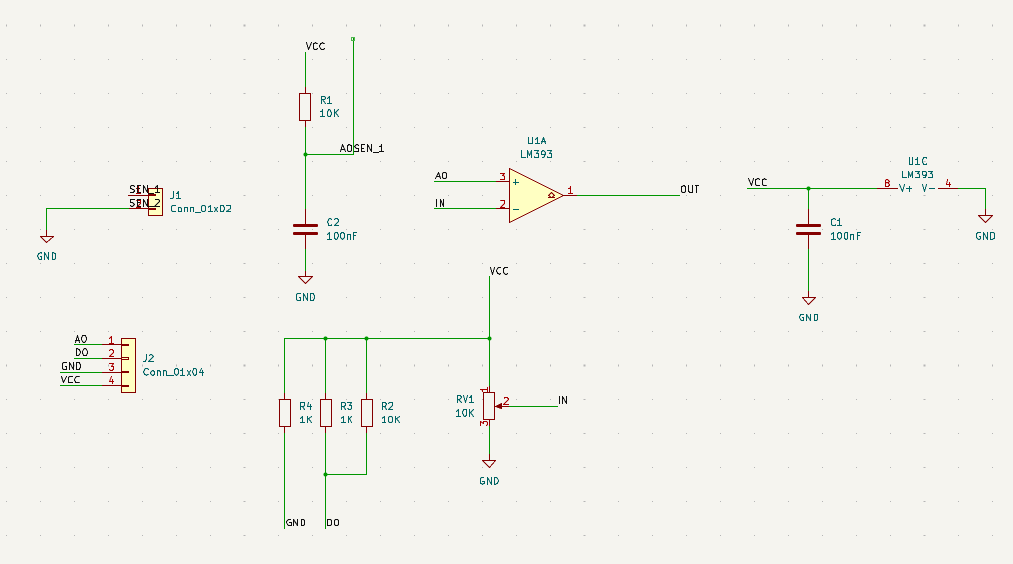
\includegraphics[width=0.8\textwidth]{Figures/FSR402_Circuit_F.png}
    \caption{FSR402 Failed Circuit}
    \label{fig:fsr402_failed_circuit}
\end{figure}
\begin{table}[h]
        \centering
        \begin{tabular}{|l|l|l|l|}
            \hline
            \textbf{PCB Type} & \textbf{Test Item} & \textbf{Expected Result} & \textbf{Actual Result} \\ \hline
            Failed& Voltage on AO & $\frac{1k\Omega}{11k\Omega}\times 3.3V=0.3V$ & 3.17V \\ \hline
            Failed& R between sensor port 2 and VCC & $10k\Omega$ & $9.792k\Omega$ \\ \hline
            Failed& R between VCC and DO & $\frac{1k\Omega\times10k\Omega}{1k\Omega+10k\Omega}\approx 909.1 \Omega$ & $6.147k\Omega$ \\ \hline
            Success& Voltage on AO & 3.3V & 3.197V \\ \hline
            Success& R between sensor port 1 and VCC & $10k\Omega$ & $9.807k\Omega$ \\ \hline
            Success& R between VCC and DO & $10k\Omega$ & $9.076k \Omega$ \\ \hline
        \end{tabular}
        \caption{PCB Testing}
        \label{tab:pcb_testing}
    \end{table}   
